\section{Probability}
\subsection{}section{Uncertainty}
We want to predict and approximate Uncertainty. 

A pure logical approach may not be fully realistic. It can lead to conclusions that are too weak for decision making. It also leads to non-optimal decisions.

We want to have a representation of uncertainty with probabilities.

\subsection{Probability}
\textbf{Sample space}: $\Omega$ is the sample space (set of possibilities). $\omega \in \Omega$ is a sample point/possible world/atomic event/outcome of a random process...

\textbf{Probability space} (or model): is a function $P: \Omega \xrightarrow[]{} R$ such that:
\begin{itemize}
    \item $0 \leq P(\omega)\leq 1$
    \item $\sum_{\omega \in \Omega} P(\omega) = 1$
\end{itemize}

\subsection{Event}
An event A is any subset of $\Omega$. \\
Probability of an event A is a function assigning to A a value [0, 1]
\begin{equation}
    P(A) = \sum_{\omega \in A} P(\omega)
\end{equation}
\subsection{Random Variables}
A \textbf{random variable} is a function from the sample space $\Omega$ to some range $X: \Omega \xrightarrow[]{}B$ \\
Example: $Odd: \Omega \xrightarrow[]{} Boolean$ \\
P introduces a probability distribution for a random variable X:
\begin{equation}
    P(X = x_{i}) = \sum_{\{\omega \in \Omega | X(\omega) = x_{i}\}} P(\omega)
\end{equation}
\subsection{Proposition}
A \textbf{proposition} is the event where an assignment to a random variable holds. Propositions can be combined using standard logical operators.
We can map functions to propositional logic.
\subsection{Syntax for proportions}
Propositional or Boolean random variables, Discrete random variables, Continuous random variables, Arbitrary Boolean combinations of basic proposition.
\subsection{Prior}
\textbf{Prior} or \textbf{unconditional} probabilities of propositions correspond to belief prior to arrival of any (new) evidence

\subsection{Probability Distribution}
A \textbf{probability distribution} is a function that assigns to each possible value of the random variable an apriori probability. The sum of all the values must be 1. Concepts of Probability distribution can be extended to continuous variables.

\subsection{Joint probability distribution}
\textbf{Joint probability distribution} for a set of random variables gives the probability of every atomic joint event of those random variables.

Joint probability distribution of two random variables is a grid where each cell is the sum of the probabilities of the event that correspond to the column and row.

\subsection{Conditional/Posterior probability}
Belief after the arrival of some evidence. I know the outcome of a random variable, how does this affect probability of other random variables?\\
$P(X=true|W=true) = ?$ \\
$P(X=true|W=true) \neq P(X=true, W=true) \neq P(X=true)$ \\
\subsubsection{Definition of conditional probability}
Conditional probability:
\begin{equation}
    P(a|b) \equiv \frac{P(a \land b)}{P(b)}\ if\ P(b) \neq 0
\end{equation}
Product rule:
\begin{equation}
    P(a \lor b) = P(a|b)P(b) = P(b|a)P(a)
\end{equation}
A general version holds for whole distributions.
\subsection{Total probabilities}

\begin{equation}
    P(a) = P(a|b)P(b) + P(a|\neg b)P(\neg b)
\end{equation}
in general, for a random variable Y accepting mutual exclusive values y:
\begin{equation}
    P(X) = \sum_{y_{i} \in D(Y)} P(X|Y=y_{i})P(Y=y_{i})
\end{equation}
D(Y): set of values for variable Y.

\subsection{Chain Rule}
\textbf{Chain rule} of derived by successive application of product rule:
\begin{equation}
    P(X_{1}, X_{2} = P(X_{1})P(X_{2}|X_{1}) \\
    P(X_{1} \dots X_{n}) = \prod_{i=1}^{n}P(X_{i}|X_{1}\dots X_{i-1})
\end{equation}

\subsection{Inference by enumeration}
\begin{figure}[H]
    \centering
    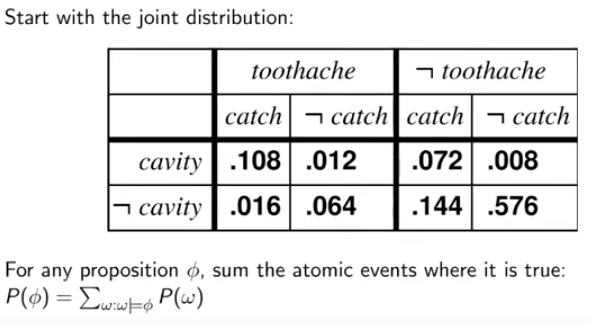
\includegraphics[width=12cm]{images/Probabilities/Inference_by_enum.png}
    \caption{}
    \label{fig:infbyenum}
\end{figure}

\subsection{Independence}
A and B are independent iff
$P(A|B) = P(A)$ or $P(B|A) = P(B)$ or $P(A, B) = P(A)P(B)$

Absolute independence is impossible.

\subsection{Conditional independence}

X is conditional independent from Y given Z iff $P(X|Y,Z) = P(X|Z)$ \\
$P(X,Y|Z) = P(X|Y,Z)P(Y|Z) = P(X|Z)P(Y|Z)$ \\

$Y_{i}$ conditional independent from $Y_{j}$ given Z:
\[P(Y_{1}\dots Y_{n}|Z) = P(Y_{1}|Z)\dots P(Y_{j}|Z)\]

Chain rule + conditional independence:
\[P(X,Y,Z) = P(X|Y,Z)P(Y,Z) = P(X|Y,Z)P(Y|Z)P(Z) = P(X|Z)P(Y|Z)P(Z)\]
\subsection{Bayes' Rule}
Product rule:
\[P(a\land b) = P(a|b)P(b) = P(b|a)P(b) = P(b|a)P(a) = \]
\[= Bayes'rule P(a|b) = \frac{P(b|a)P(a)}{P(b)}\]

\subsection{Bayesian networks}

Graphical notation for conditional independence assertions and hence for compact specification of full joint distributions.\\
Syntax:
\begin{enumerate}
    \item a set of nodes, one per variable
    \item a direct, acyclic graph
    \item a conditional distribution for each node given its parents 
\end{enumerate}
represented as a conditional probability table (CPT) giving the distribution over $X_{i}$ for each combination of parent values
